\documentclass[twocolumn]{article}
\usepackage{preamble}
% \usepackage{fullpage}
\usepackage{dsfont}
\usepackage{algorithm}
\usepackage{algorithmic}
\usepackage{paralist}
\usepackage{csvsimple}
\usepackage{longtable}
\usepackage{booktabs}
\usepackage{tikz}
\usepackage{afterpage}

\sisetup{range-phrase=-}


\newcommand{\drawfrom}{\overset{\mathrm{d}}{=}}
\newcommand{\setfrom}{\overset{\mathrm{d}}{\leftarrow}}

\title{ \small
University of Oslo\\
FYS4411\\
Computational physics II: Quantum mechanical systems\\
\huge Project 1 }
\author{\textsc{Bendik Samseth}}
\date{\today}
\begin{document}
\maketitle


\section{Introduction}
The aim of this project is to use the Variational Monte Carlo
(VMC) method and evaluate the ground state energy of a trapped, hard
sphere Bose gas for different numbers of particles with a specific
trial wave function. This trial wave function is used to study the sensitivity of
condensate and non-condensate properties to the hard sphere radius
and the number of particles.  

\section{Theory}
\subsection{Physical System}
\textbf{The trap} we will use is a spherical (S)
or an elliptical (E) harmonic trap in one, two and finally three
dimensions, with the latter given by

\begin{equation}
    V_{ext}(\mathbf{r}) = 
    \Bigg\{
        \begin{array}{ll}
            \frac{1}{2}m\omega_{ho}^2r^2 & (S)\\
            \strut
            \frac{1}{2}m[\omega_{ho}^2(x^2+y^2) + \omega_z^2z^2] & (E)
            \label{trap_eqn}
        \end{array}
\end{equation}
\textbf{The Hamiltonian} of the system will be
\begin{equation}
    H = \sum_i^N \left(\frac{-\hbar^2}{2m}{\bigtriangledown }_{i}^2 +V_{ext}({\mathbf{r}}_i)\right)  +
     \sum_{i<j}^{N}
     V_{int}({\mathbf{r}}_i,{\mathbf{r}}_j),\label{eq:Hamiltonian}
\end{equation}
Here $\omega_{ho}^2$ defines the trap potential strength.  In the case of the
elliptical trap, $V_{ext}(x,y,z)$, $\omega_{ho}=\omega_{\perp}$ is the trap
frequency in the perpendicular or $xy$ plane and $\omega_z$ the frequency in
the $z$ direction.  The mean square vibrational amplitude of a single boson at
$T=0K$ in the trap (\ref{trap_eqn}) is $\langle
x^2\rangle=(\hbar/2m\omega_{ho})$ so that $a_{ho} \equiv
(\hbar/m\omega_{ho})^{\frac{1}{2}}$ defines the characteristic length of the
trap.  The ratio of the frequencies is denoted
$\lambda=\omega_z/\omega_{\perp}$ leading to a ratio of the trap lengths
$(a_{\perp}/a_z)=(\omega_z/\omega_{\perp})^{\frac{1}{2}} = \sqrt{\lambda}$.

\vspace{0.3cm}\hrule\vspace{0.2cm}
Note: In the rest of this report, as well as in accompanying source code, we
will use natural units with $\hbar = m = 1$.
\vspace{0.2cm}\hrule\vspace{0.3cm}

We will represent \textbf{the inter-boson interaction} by a pairwise,
repulsive potential:
\begin{equation}
    V_{int}(|\mathbf{r}_i-\mathbf{r}_j|) =  \Bigg\{
        \begin{array}{ll}
            \infty & {|\mathbf{r}_i-\mathbf{r}_j|} \leq {a}\\
            0 & {|\mathbf{r}_i-_r\mathbf{r}_j|} > {a}
        \end{array}
\end{equation}
where $a$ is the so-called hard-core diameter of the bosons.
Clearly, $V_{int}(|\mathbf{r}_i-\mathbf{r}_j|)$ is zero if the bosons are
separated by a distance $|\mathbf{r}_i-\mathbf{r}_j|$ greater than $a$ but
infinite if they attempt to come within a distance $|\mathbf{r}_i-\mathbf{r}_j| \leq a$.

\textbf{The trial wave function} for the ground state with $N$ atoms will be given by
\begin{align}
    \begin{split}
    \Psi_T(\mathbf{r})&=\Psi_T(\mathbf{r}_1, \mathbf{r}_2, \dots
    \mathbf{r}_N,\alpha,\beta)\\
    &=\prod_i g(\alpha,\beta,\mathbf{r}_i)\prod_{i<j}f(a,|\mathbf{r}_i-\mathbf{r}_j|),
    \end{split}
    \label{eq:trialwf}
\end{align}
where $\alpha$ and $\beta$ are variational parameters. We choose the
single-particle wave function to be proportional to the harmonic
oscillator function for the ground state, i.e., we define $g(\alpha,\beta,\mathbf{r}_i)$ as:
\begin{equation}
    g(\alpha,\beta,\mathbf{r}_i)= \exp[-\alpha(x_i^2+y_i^2+\beta z_i^2)].
\end{equation}
For spherical traps we have $\beta = 1$ and for non-interacting
bosons ($a=0$) we have $\alpha = 1/2a_{ho}^2$ resulting in the exact wave
function. The correlation wave function is

\begin{equation}
    f(a,|\mathbf{r}_i-\mathbf{r}_j|)=\Bigg\{
        \begin{array}{ll}
            0 & {|\mathbf{r}_i-\mathbf{r}_j|} \leq {a}\\
            (1-\frac{a}{|\mathbf{r}_i-\mathbf{r}_j|}) & {|\mathbf{r}_i-\mathbf{r}_j|} > {a}.
        \end{array}
\end{equation}

\subsubsection{Scaling the System}

We will use distances in units of $a_{ho}$ in this report, $\vec r'=\vec r /a_{ho}$.
Performing this substitution in the Hamiltonian \eqref{eq:Hamiltonian}, using
$\nabla^{\prime 2} = a_{ho}^2\laplacian$, we get:
\begin{align*}
    H &= \sum_i^N\qty(-\frac{\hbar^2}{2m}\laplacian_i + V_{ext}(\vec r_i)) +
    \sum_{i<j}^NV_{int}(\vec r_i, \vec r_j)\\
    &= \sum_{i}^N\left(-\frac{\hbar^2}{2m}
    \frac{1}{a_{ho}^2}\nabla_i^{\prime 2}\right.\\
    &\,
    \qqtext{  }\qqtext{
    }+\left.\frac{m}{2}\qty[\omega_{ho}^2a_{ho}^2\qty(x_i^{\prime 2} +
    y_i^{\prime 2}) +
    \omega_z^2a_{ho}^2z_i^{\prime 2}]\right)\\
    &\,
    \qqtext{  }+ \sum_{i<j}^NV_{int}(\vec r_i, \vec r_j)\\
    \begin{split}
        &= \frac{\hbar\omega_{ho}}{2}\sum_{i}^N\qty(-\nabla_i^{\prime 2} +
        x_i^{\prime 2} + y_i^{\prime 2} + \lambda^2z_i^{\prime 2})\\
    &\,\qqtext{  }+ \sum_{i<j}^NV_{int}(\vec r_i, \vec r_j)
    \end{split}\numberthis\label{eq:Hamiltonian-scaled}
\end{align*}
where once again $\lambda = \flatfrac{\omega_z}{\omega_{ho}}$ describes the
asymmetry in the trap. The interaction potential remains the same, as all
lengths are scaled, and only the relative distances are used. 

There will also be a scaling factor for the single-particle wave functions, 
\begin{align}
    g(\alpha, \beta, \vec r_i) = \exp[-\alpha a_{ho}^2(x_i^{\prime 2} +
    y_i^{\prime 2} + \beta z_i^{\prime 2})].
\end{align}
The correlation wave functions remains unaffected.

All energies will due to this be given in units of $\hbar\omega_{ho}$, and
lengths in units of $\alpha_{ho}$. We fix the value of $\omega_{ho}=1$ so that,
along with the use of the natural units of $\hbar=m=1$, we have 
\begin{align}
    a_{ho} = \sqrt{\frac{\hbar}{m\omega_{ho}}} = 1.
\end{align}

This means the scaling has no effect on the numbers we would get, but now we
have a well defined scale to relate the numbers to.

For notational sanity, the use of ticks to denote the scaled variables will be
omitted, and can be assumed in the remainder of this report. 



\subsection{The Objective}
Our objective is to evaluate the expectation value of the Hamiltonian. We cannot do this
without the true wave function of the system, something we do not possess.
We can, however, approximate the energy with the trial wave function.
\begin{align}
    E[H] = \expval{H} = \frac{\int \dd{\vec R} \Psi^*_T H \Psi_T}{\int
    \Psi_T^*\Psi_T}.
\end{align}
where $\vec R$ is the matrix containing all the positions of the particles in
the system, $\vec R = [\vec r_1, \vec r_2, \dots, \vec r_N]$.
In order to numerically evaluate this integral we first manipulate it a bit.
The probability density at position $\vec R$, under the trial wave function, is
\begin{align}
    P(\vec R, \vec \alpha) &= \frac{\abs{\Psi_T}^2}{\int \dd{\vec R}\abs{\Psi_T}^2}.
\end{align}
where $\vec \alpha$ is used for shorthand and represents the vector of all the variational parameters.
We finally define a new quantity, called \textbf{the local energy}:
\begin{align}
    E_L(\vec R, \vec \alpha) &= \frac{1}{\Psi_T}H\Psi_T\label{eq:E_L}
\end{align}
Combining these two definitions we can now rewrite $\expval{H}$ as follows:
\begin{align}
    \begin{split}
        \expval{H} &= \int \dd{\vec R} P(\vec R,\vec\alpha) E_L(\vec R,\vec\alpha)\\
        &\approx
        \frac{1}{N}\sum_{i=1}^N E_L(\vec R_i,\vec\alpha),
    \end{split}\label{eq:the-objective}
\end{align}
where $R_i$ are randomly drawn positions from the PDF $P(\vec R, \vec\alpha)$.
We have therefore that estimating the average value of $E_L$ yields an
approximated value for $\expval{H}$. This value is in turn be an upper bound on the
ground state energy, $E_0$. By the variational principle, if we minimize
$\expval{H}$ under the variational parameters, we find an estimate for the true
ground state energy of the system.

\subsubsection{Exact Result for Simple System}

It will be useful to be able to compare our results with exact analytical
results where we have these. In the case of the symmetric harmonic oscillator
trap, ignoring any iteractions between the bosons, we have an exact form for the
ground state energy:
\begin{align}
    E_0 = \sum_{i=1}^N\sum_{d=1}^{D=\{1,2,3\}} \frac{\hbar \omega_{ho}}{2} 
    = \frac{N\times D}{2},\label{eq:exact-ground-state}
\end{align}
for $N$ independent bosons in $D$ dimensions (the two sums goes
over all the degrees of freedom in the system). This follows from the setting
$\alpha=\flatfrac{1}{2}$ (and $\beta=1$) in $\Psi_T$, and using $a=0$ (no
interaction). 

We also have an exact value for the variance of the energy in this case:
\begin{align}
    \begin{split}
        \sigma_E^2 &= \expval{H^2} - \expval{H}^2\\
            &= \expval{H^2}{\Psi}-\expval{H}{\Psi}^2\\
            &= \expval{E^2}{\Psi}-\expval{E}{\Psi}^2\\
            &= E^2\braket{\Psi} - \qty(E\braket{\Psi})^2= 0.
    \end{split}\label{eq:var-zero-when-exact}
\end{align}
This follows when we have the exact wavefunction, which satisfies the time
independent Schrödinger equation, $H\ket{\Psi}=E\ket{\Psi}$.

\subsection{Calculating the Local Energy $E_L$}
As the local energy is the quantity we are interested in computing for a
large set of positions we would do well to consider how best to evaluate this
expression effectively. For this we have two alternative approaches,
\begin{inparaenum}[1)]
    \item numerical differentiation and
    \item finding an analytic, direct expression.
\end{inparaenum}

\subsubsection{Numerical differentiation}
We may set up an algorithm for the numerical approximation of the local energy
as shown in Algorithm~\ref{alg:E_L-numeric}.
\begin{algorithm}[H]
    \caption{Calculate the local energy $E_L$ using numerical differentiation.}
    \label{alg:E_L-numeric}
    \begin{algorithmic}[1]
        \REQUIRE $\vec R = [\vec r_1,\vec r_2,\dots,\vec r_N]$, $D=\text{dimensions}$
        \ENSURE $y = E_L$
        \STATE $y = -2\times N\times D\times  \Psi_T(\vec R)$
        \FOR{$i = 1$ \TO $N$}
            \FOR{$d = 1$ \TO $D$}
                \STATE $\vec R_+\leftarrow \vec R + h \vec e_{i, d}$
                \STATE $\vec R_-\leftarrow \vec R - h \vec e_{i, d}$
                \STATE $y\leftarrow y + \Psi_T(\vec R_+) + \Psi_T(\vec R_-)$
            \ENDFOR
        \ENDFOR
        \STATE $y\leftarrow -\flatfrac{y}{2h^2}$
        \STATE $y\leftarrow \flatfrac{y}{\Psi_T(\vec R)}+\sum_{i=1}^N V_{ext} + \sum_{i<j}^N V_{int} $
    \end{algorithmic}
\end{algorithm}
An evaluation of $E_L$ using this algorithm would be $\mathcal{O}(N^3\times
D)=\mathcal{O}(N^3)$ with interaction, and $\mathcal{O}(N^2)$ without interaction, from
the complexity of $\Psi_T$.



\subsubsection{Finding an Analytical Expression for $E_L$}
Straight forward numerical differentiation is of course an
option, but this is likely to be quite time-expensive to do. We will here try to
speed up the calculation by producing a direct formula.

The hard part of the expression for $E_L$ is
\begin{align}
    \frac{1}{\Psi_L}\sum_{k}^N\laplacian_k{\Psi_L}.
\end{align}
To get going, we rewrite the wave function as
\begin{align}
    \Psi_L(\vec R) &= \prod_i \phi(\vec r_i)\exp(\sum_{i<j}u(r_{ij})),
\end{align}
where $r_{ij} = \norm{\vec r_{ij}} = \norm{\vec r_i - \vec r_j}$, $u(r_{ij}) =
\ln f(r_{ij})$, and $\phi(\vec r_i)=g(\alpha,\beta,\vec r_i)$.

Lets first evaluate the gradient with respect to particle $k$
\begin{align}
    \begin{split}
    \grad_k{\Psi_T(\vec r)}  
    &= \grad_k{\prod_i \phi(\vec r_i)\exp(\sum_{i<j}u(r_{ij}))}\\
    &= \prod_{i\neq k} \phi(\vec r_i)\exp(\sum_{i<j}u(r_{ij}))\grad_k{\phi(\vec
    r_k)}\\
    &+ \prod_{i} \phi(\vec r_i)\grad_k{\exp(\sum_{i<j}u(r_{ij}))}\\
    &= \Psi_T\qty[\frac{\grad_k \phi(\vec r_k)}{\phi(\vec r_k)} + \sum_{j\neq k}
    \grad_k u(r_{kj})].
    \end{split}\label{eq:grad-trail-wf}
\end{align}
The first term is evaluated quite simply:
\begin{align}
    \begin{split}
    \frac{\grad_k\phi(\vec r_k)}{\phi(\vec r_k)} &= \frac{\grad_k}{\phi(\vec r)}
    \exp[-\alpha\qty(x_k^2 + y_k^2 + \beta z_k^2)]\\
        &= -2\alpha\hat{\vec r}_k,
    \end{split}\label{eq:grad-phi_k-over-phi_k}
\end{align}
where the notation $\hat{\vec r}_k = (x, y,\beta z)$ is introduced for brevity.
Note that in the 1D and 2D case we simply have $\hat{\vec r}_k = \vec r_k$.


The second term may be evaluated as follows:
\begin{align}
    \begin{split}
    \grad_k u(r_{kj}) &= u'(r_{kj})\grad_k \sqrt{\norm{\vec r_k - \vec r_j}^2} \\
    &= \frac{u'(r_{kj})}{2r_{kj}}\grad_k\qty(\norm{\vec r_k}^2-2\vec r_k\vdot\vec
    r_j+\norm{r_j}^2)\\
    &= u'(r_{kj})\frac{\vec r_{kj}}{r_{kj}}\\
    &= \pdv{}{r_{kj}}\qty[ \ln(1 - \frac{a}{r_{kj}})] \frac{\vec
    r_{kj}}{r_{kj}}\\
    &= \frac{\vec r_{kj}}{r_{kj}}\frac{a}{r_{kj}(r_{kj}-a)}.
    \end{split}\label{eq:grad-u}
\end{align}

Now we can find the Laplacian by taking the divergence of
\eqref{eq:grad-trail-wf}:
\begin{align*}
\frac{1}{\Psi_L}\laplacian_k{\Psi_L} &= \frac{1}{\Psi_L}\grad_k\vdot
    \Psi_T\qty[\frac{\grad_k \phi(\vec r_k)}{\phi(\vec r_k)} + \sum_{j\neq k}
    \grad u(r_{kj})] \\
    &= \frac{\laplacian_k \phi(\vec r_k)}{\phi(\vec r_{k})}+\sum_{j\neq
    k}\laplacian_k u(r_{kj})\\
    &+ \frac{\grad_k\qty(\phi(\vec r_k)) \vdot \qty(\sum_{j\neq k} \grad_k
    u(r_{kj}))}{\phi(\vec r_k)}\\
    &+ \left[
        \qty(\frac{\grad_k \phi(\vec r_{k})}{\phi(\vec r_k)} 
        + \sum_{j\neq k}\grad_k u(r_{kj})    )\right.\\
        &\left.\vdot
        \qty(\sum_{j\neq k} \grad_k u(r_{kj})   )\right] \\
    &= \frac{\laplacian_k \phi(\vec r_k)}{\phi(\vec r_k)}
    + 2 \frac{\grad_k \phi(\vec r_k)}{\phi(\vec r_k)}\vdot
    \sum_{j\neq k}\qty( \frac{\vec r_{kj}}{r_{kj}}u'(r_{kj}))\\
    &+ \sum_{i,j \neq k} \frac{\vec r_{ki}\vdot\vec r_{kj}}{r_{ki}r_{kj}}
    u'(r_{ki})u'(r_{kj})
    + \sum_{j\neq k}\laplacian_k u(r_{kj}).\numberthis\label{eq:almost-done-EL}
\end{align*}
There are two new quantities here which need to be evaluated before we are done:
\begin{align}
    \begin{split}
    \frac{\laplacian_k \phi(\vec r_k)}{\phi(\vec r_k)} &=
    2\alpha\qty[2\alpha \norm{\hat{\vec r}_k}^2 - d(\beta)],\\
    &\text{with } d(\beta) = \begin{cases}
        1 &\qfor \text{1D}\\
        2 &\qfor \text{2D}\\
        2 + \beta &\qfor \text{3D}
    \end{cases},
    \end{split}
\end{align}
and
\begin{align}
    \begin{split}
    \laplacian_k u(r_{kj}) &= \grad_k\vdot u'(r_{kj})\frac{\vec
    r_{kj}}{r_{kj}} \\
    &= u'(r_{kj})\frac{2}{r_{kj}} + \frac{\vec r_{kj}}{r_{kj}}\vdot \grad_k
    u'(r_{kj})\\
    &= u''(r_{kj}) + \frac{2}{r_{kj}}u'(r_{kj}),
    \end{split}
\end{align}
where
\begin{align}
    \begin{split}
    u''(r_{ij}) &= \pdv[2]{}{r_{ij}} \ln(1-\frac{a}{r_{ij}})\\
    &= \frac{a(a-2r_{ij})}{r_{ij}^2(r_{ij}-a)^2}.
    \end{split}
\end{align}

Inserting all of this back into \eqref{eq:almost-done-EL} we get:
\begin{align}
    \begin{split}
    \frac{1}{\Psi_L}\laplacian_k{\Psi_L} &=  
    2\alpha\qty[2\alpha \norm{\hat{\vec r}_k}^2 - d(\beta)]\\
    &- 4\alpha\hat{\vec r}_k \vdot
    \qty[ \sum_{j\neq k} \frac{\vec r_{kj}}{r_{kj}}
    \frac{a}{r_{kj}(r_{kj}-a)}]\\
    &+  \sum_{i,j\neq k} \frac{\vec r_{ki}\vdot\vec r_{kj}}{r_{ki}r_{kj}}
    \frac{a}{r_{ki}(r_{ki}-a)}\frac{a}{r_{kj}(r_{kj}-a)}\\
    &+ \sum_{j\neq k} \qty(
    \frac{a(a-2r_{kj})}{r_{kj}^2(r_{kj}-a)^2} +
    \frac{2}{r_{kj}}\frac{a}{r_{kj}(r_{kj}-a)}).
    \end{split} \label{eq:E_L-part-final}
\end{align}
We may note that without interactions ($a=0$), this simplifies to only the first
term, as all the other terms are proportional to $a$.

The complete expression for the local energy is then:
\begin{align*}
    E_L &= \frac{1}{\Psi_T}H\Psi_T\\
    &= \sum_{i}V_{ext}(\vec r_i) + \sum_{i<j}V_{int}(\vec r_i,\vec r_j)
    - \frac{1}{2}\sum_k
    \frac{1}{\Psi_T}\laplacian_k\Psi_T\numberthis\label{eq:E_L-final}
\end{align*}
where we substitute in \eqref{eq:E_L-part-final} in the final sum. A single
evaluation of the local energy is then $\mathcal{O}(N^3)$ with interaction,
and $\mathcal{O}(N)$ without.

We can see that without interaction we obtain a linear-time expression, compared
to quadratic-time using numerical differentiation. With interaction we have
not been able to improve the complexity in terms of Big-O. This does not,
however, mean that no improvement is obtained. A closer look shows that the
numerical approach uses more evaluations by a constant factor of about three.
This stems from the three wave function evaluations used in the central
difference approximation of the second derivative. The analytic approach is
closer to using a single evaluation, although the exact ratio is hard to define
as the wave function is not directly used here.

In summary, we will expect a significant speedup using the analytic expression
both with and without interaction enabled. 


\subsection{Calculating the Quantum Drift Force}
Anticipating its later use, we will also find an expression for the so called
quantum drift force, which we shall use when we consider importance sampling.
For now, we just give its definition:
\begin{align}
    \vec F_k = \frac{2\grad_k\Psi_T}{\Psi_T}\label{eq:Q-force-def}
\end{align}
This is interpreted as the force acting on particle $k$ due to the trap and/or
presence of other particles. As a physical justification for why $\vec F_k$
takes this form we can see that $\vec F_k$ is
proportional with the gradient of $\Psi_T$, which we can intuitively understand
as a force pushing the particle towards regions of space with higher
probability. 

Luckily this can now be quickly evaluated due to
the results of the previous section,
\begin{align}
    \vec F_k = 2\qty[\sum_{j\neq k}\frac{\vec r_{kj}}{r_{kj}}
    \frac{a}{r_{kj}(r_{kj}-a)} - 2\alpha\hat{\vec
    r}_k].\label{eq:Q-force-explicit}
\end{align}
With interaction this is $\mathcal{O}(N)$, and without ($a=0$) it simplifies to $\mathcal{O}(1)$.

For brevity, we may later use the notation $\vec F(\vec R) = [\vec F_1, \vec
F_2,\dots,\vec F_N]$, denoting the matrix of all the individual forces on each
particle.

\subsection{One-Body Density}

A quantity which is often of great interest is the one-body density. It is defined for particle $1$ as
\begin{align}
    \rho(\vec r_1) = \int \dd{\vec r_2}\dd{\vec r_3}\dots\dd{\vec r_N} \abs{\Psi(\vec R)}^2\label{eq:one-body-def},
\end{align}
and similarly for particle $i = 2,3\dots, N$. All particles are indistinguishable, so which $i$ we consider is arbitrary.

The one-body density gives a measure of the distribution of particles in the
system. It can be read as: if we marginalize out the positions of all other
particles, what is the likelihood of finding particle $i$ in a given position?
The answer to this question is given by $\rho_(r_i)$.

For the non-interacting case we can evaluate this expression exactly, as the
wavefunction separates nicely.
\begin{align}
    \begin{split}
        \rho(\vec r_k)&=g(\vec r_k)\prod_{i\neq k}\iiint_{-\infty}^\infty
        \dd{x_i}\dd{y_i}\dd{z_i}g(\vec r_i)\\
        &= \qty(\frac{\pi^{3/2}}{2\sqrt{2}\alpha^{3/2}\sqrt{\beta}})^{N-1}
        g(\vec r_k)\\
    \end{split}\label{eq:one-body-exact}
\end{align}
The constant is of little importance to us, but what we want is the functional
form of $\rho(\vec r_k$, which we see follows the Gaussian shape of the
single-particle wavefunction.

In the non-interacting case this integral is far less friendly to us, and we have no
exact formula or shape. We shall therefore compute the integral numerically. However, 
instead of going about this with straight forward Monte Carlo integration, we
shall take a more intuitive approach.

We split the position space into $M$ spheres\footnote{Or circles in 2D, and line
segments in 1D.} of increasing radii, $r_i=i * r_\text{step}$ for $i=1,\dots,M$,
all centered at the origin. The volume of the sphere with radius $r_{i+1}$, minus
the volume of the sphere with radius $r_i$, we call region $i+1$. The
illustration below shows this graphically, where region $i+1$ is the lightly
shaded region.

\begin{center}
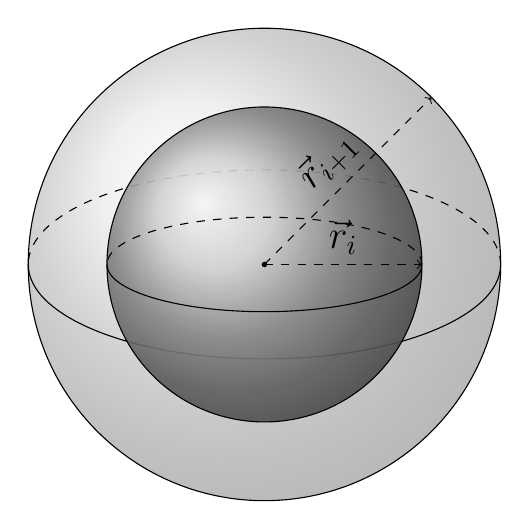
\begin{tikzpicture}
  \shade[ball color = gray!40, opacity = 0.4] (0,0) circle (3cm);
  \draw (0,0) circle (3cm);
  \draw (-3,0) arc (180:360:3 and 1.2);
  \draw[dashed] (3,0) arc (0:180:3 and 1.2);
  \fill[fill=black] (0,0) circle (1pt);

  \shade[ball color = gray!50, opacity = 0.9] (0,0) circle (2cm);
  \draw (0,0) circle (2cm);
  \draw (-2,0) arc (180:360:2 and 0.6);
  \draw[dashed] (2,0) arc (0:180:2 and 0.6);
  \fill[fill=black] (0,0) circle (1pt);
  \draw[dashed, ->] (0,0 ) -- node[above]{\Large $\vec r_i$} (2,0);
  \draw[dashed, ->] (0,0 ) -- node[sloped, anchor=center, above]{\Large $\vec r_{i+1}$} (2.1213,2.1213);
\end{tikzpicture}
\end{center}

For each sampled position $\vec R$, we can note down which region particle $1$
(arbitrary choice) is within, and keep a running tally for each region. After
sampling many positions, we normalize each region count by both the number of
samples and the volume\footnote{Or area in 2D, and length in 1D} of the
region. Given a small enough $r_\text{step}$, and enough samples, we would then
plot the normalized region counts against their radii, and this would be expected
to approximate the one-body density well.

As a technical note, because the choice of which particle we observe is
arbitrary, we could have done this for any other particle. We could therefore do
it for all particles in parallel, by noting which region \textit{every} particle
lands in. Since they should all produce a similar result, we could average the
recorded counts across all particles. This should be roughly the same as if we
had $N$ times as many samples and only counted for one particle.


\section{Algorithms}
In \eqref{eq:the-objective} we reformulated our objective of estimating the ground state energy of the
system, $\expval{H}$, to minimizing the average local energy, $\expval{E_L(\vec \alpha)}$ w.r. to
the variational parameters $\vec \alpha = (\alpha, \beta)$. Key to this
reformulation was that the local energy had to be sampled with positions $\vec
R$ that where drawn from the PDF $P(\vec R, \vec\alpha)$. As $P$ is far from any
standard PDF with a known inverse CDF, we cannot trivially generate such
samples. In addition, the normalisation term in its denominator is
computationally expensive to compute. These limitations make the
\textit{Metropolis algorithm} the obvious choice to solve this problem. This
algorithm provides a way to generate random samples from a PDF where we only
know the probabilities up to a proportionality constant.

\subsection{Metropolis Algorithm}
The algorithm in its
simplest form is described in Algorithm~\ref{alg:metropolis-simple}.

\begin{algorithm}[H]
    \caption{The Metropolis algorithm in its simplest form, as it
    pertains to our specific application.}
    \label{alg:metropolis-simple}
    \begin{algorithmic}[1]
        \REQUIRE $M$, generates $M\times N$ samples.
        \ENSURE $\text{samples} \setfrom P(\vec R, \vec\alpha)$
        \STATE $\text{samples} \leftarrow \text{empty list}$
        \STATE $\vec R \leftarrow \text{randomly initialized matrix of positions}$
        \FOR{$M$ iterations}
            \FOR{every particle $i\in[1, N]$}
                \STATE $\Delta \vec{r} \leftarrow \text{random perturbation vector}$
                \STATE $\vec R^*\leftarrow \vec R $
                \STATE $\vec R^*_i \leftarrow \vec R^{*}_i+ \Delta \vec{r}$ 
                \STATE $q \leftarrow \flatfrac{\abs{\Psi_T(\vec R^*)}^2}{\abs{\Psi_T(\vec R)}^2}$
                \STATE $r \setfrom \text{Unif}(0, 1)$
                \IF{ $r\leq q$ }
                    \STATE $\vec R \leftarrow \vec R^*$
                \ENDIF
                \STATE Append $\vec R$ to samples
            \ENDFOR
        \ENDFOR
    \end{algorithmic}
\end{algorithm}

In this algorithm we move around in position space randomly, accepting new
positions biased towards areas of space where $P(\vec R,\vec\alpha)$ is higher.
We choose to move one particle at a time based on computational efficiency, as
recalculating the local energy can be done more easily when we know only one
particle has moved\footnote{Not actually implemented yet.}.

With the generated list of positions we may produce and average for the local
energy, and therefore an estimate for an upper bound on the ground state energy,
as well as the one-body density, or any other quantity of interest.

\subsubsection{Limitations}
This algorithm has two major drawbacks. Firstly, the samples generated are not
independent. It is quite clear from the algorithm that the probability of
drawing a certain position is highly dependent on what position we were at
previously. The has implications on how we perform our statistical analysis, as
we must attempt to correct for this limitation. More on this in
section~\ref{sec:statistical-analisys}.

Secondly this algorithm will be quite ineffective in that a significant portion
of the suggested moves (new positions, $\vec R^*$ in
Algorithm~\ref{alg:metropolis-simple}) will be rejected. This is because the new
positions are generated at random, which might cause us to wander around in
regions of position space that are of very little significance, and it might
take a while before we (by chance) stumble upon a more high-probability region.
The effect is then a list of samples that may not be an accurate representation
of the PDF we were trying to approximate to begin with. This will be especially
true for smaller sample sizes, were these defects will account for a larger
proportion of the samples.


\subsection{Metropolis-Hastings Algorithm - Including Importance Sampling}
The first limitation of the simple algorithm (not i.i.d.) is inherent to this
kind of sampling, and is hard to avoid. We may, however, attempt to remedy the
second limitation by guiding the random walker towards more promising regions of
position space by proposing new positions in a smarter way than purely randomly.

\subsubsection{Physical Motivation of Results}
We will limit our selfs to a superficial derivation, focusing only on giving a
physical motivation for the results we end up using, as it is outside the scope
of this project to derive this rigorously.

\paragraph{Better generation of new positions:}$\,$\\
A reasonable assumption is to say that particles will tend towards regions of
space where $\abs{\Psi_T}^2$ is larger. We may say that this is the result of a
force, namely the quantum drift force given in \eqref{eq:Q-force-def}, as we
know this force pushes particles towards regions where $\Psi_T$ is large. In
addition, as this a quantum system, we expect some degree of random motion as
well. This intuitive view is exactly what is described by
the Langevin equation,
\begin{align}
    \pdv{\vec r_k}{t} = D\vec F_k(\vec r_k) + \vec\eta,\label{eq:Langevin}
\end{align}
which describes how the position of a particle changes with time under the
influence of a drift force and random impulses. Here, $D$ is
a constant scalar referred to as the drift coefficient. We set
$D=\flatfrac{1}{2}$, originating from the same factor in the kinetic energy. The
term $\vec\eta$ is a vector of
uniformly distributed random values, giving the particle some random motion in each
dimension.

Solving the Langevin equation we can obtain new positions at some time
$t+\Delta t$. Using Euler's method we get:
\begin{align}
    \vec r^* = \vec r + \frac{1}{2}\vec F_k(\vec r_k)\Delta t + \vec \xi\sqrt{\Delta
    t}\label{eq:Langevin-solution},
\end{align}
given a time step $\Delta t$, and where $\vec \xi$ is the normally distributed
equivalent of $\vec \eta$. 

\paragraph{Adjusting the acceptance probability:}$\,$\\
In Algorithm~\ref{alg:metropolis-simple} the acceptance probability for a new
position $\vec R^*$ was
\begin{align}
    q(\vec R^*, \vec R) = \frac{\abs{\Psi_T(\vec R^*)}^2}{\abs{\Psi_T(\vec
    R)}^2}\label{eq:q-simple}.
\end{align}
This was based on the transition probability for going to $\vec R^*$ from $\vec
R$ being uniform. When the transition probabilities are different depending on 
where we are and where we want to go, the acceptance probability has to be
modified in order for the algorithm to work as advertised. In general, we have 
the following form for $q(\vec R^*, \vec R)$ in our case:
\begin{align}
    q(\vec R^*, \vec R) &= \frac{T_{j\rightarrow i}}{T_{i\rightarrow j}}\frac{\abs{\Psi_T(\vec R^*)}^2}{\abs{\Psi_T(\vec
    R)}^2},\label{eq:q-full}
\end{align}
where $T_{i\rightarrow j}$ is the transition probability from the original state
$i$ into the new state $j$. We see that a uniform transition probability gives
us back \eqref{eq:q-simple}. We need therefore an expression for the transition
probabilities when we use the improved generation of new positions.


To this end, we consider the \textit{Fokker-Planck} equation, which for one
dimension and one particle can be written as
\begin{align}
    \pdv{\Psi_T}{t} = D\pdv{}{x}\qty(\pdv{}{x} - F)\Psi_T,\label{eq:Fokker-Planck}
\end{align}
which describes the time-evolution of a probability distribution under the
influence of a drift force and random impulses. We let $\Psi_T$ play the role of the
probability distribution. The factor $D$ is as before, and $F$ is here the
one-dimensional, one-particle analog to $\vec F$. In
fact, this equation is the origin of the specific form of $\vec F$ presented in
\eqref{eq:Q-force-def}. 

Equation \eqref{eq:Fokker-Planck} yields a solution given by
the following Green's function (for one particle):
\begin{align}
    G(\vec r_k^*, \vec r_k, \Delta t) &\propto 
    \exp[- \frac{\norm{\vec r_k^* - \vec r_k - D\Delta t \vec F_k(\vec r_k)}^2}{4D\Delta t} ].
\end{align}
This is interpreted as the probability of transitioning to position $\vec r_k^*$
from position $\vec r_k$ in a time interval $\Delta t$. Replacing the transition
probabilities in Equation~\eqref{eq:q-full} we get the new acceptance
probability:
\begin{align}
    q(\vec R^*, \vec R) &= \frac{G(\vec r_k, \vec r_k^*, \Delta t)}{G(\vec r_k^*, \vec r_k, \Delta t)}\frac{\abs{\Psi_T(\vec R^*)}^2}{\abs{\Psi_T(\vec
    R)}^2},\label{eq:q-full-final}
\end{align}



\subsubsection{Improved Algorithm}
We are now ready to present the proper Metropolis-Hastings algorithm, with
importance sampling used to increase the number of accepted transitions.

\begin{algorithm}[H]
    \caption{The Metropolis-Hastings algorithm, as it
    pertains to our specific application.}
    \label{alg:metropolis-importance}
    \begin{algorithmic}[1]
        \REQUIRE $M$, generates $M\times N$ samples.
        \ENSURE $\text{samples} \setfrom P(\vec R, \vec\alpha)$
        \STATE $\text{samples} \leftarrow \text{empty list}$
        \STATE $\vec R \leftarrow \text{randomly initialized matrix of positions}$
        \FOR{$M$ iterations}
            \FOR{every particle $i\in[1, N]$}
                \STATE $\Delta\vec r_i^* \leftarrow \frac{1}{2}\vec
                F_i(\vec r_i)\Delta t + \vec \xi\sqrt{\Delta t}$
                \STATE $\vec R^*\leftarrow \vec R $
                \STATE $\vec R^*_i \leftarrow \vec R^{*}_i+ \Delta \vec r_i^*$ 
                \STATE $q \leftarrow \flatfrac{\abs{\Psi_T(\vec R^*)}^2}{\abs{\Psi_T(\vec R)}^2}$
                \STATE $q \leftarrow q \times \flatfrac{G(\vec r_k, \vec r_k^*,
                    \Delta t)}{G(\vec r_k^*, \vec r_k, \Delta t)}$
                \STATE $r \setfrom \text{Unif}(0, 1)$
                \IF{ $r\leq q$ }
                    \STATE $\vec R \leftarrow \vec R^*$
                \ENDIF
                \STATE Append $\vec R$ to samples
            \ENDFOR
        \ENDFOR
    \end{algorithmic}
\end{algorithm}


\section{Evaluating the Validity of Results}
\label{sec:statistical-analisys}

Once one of the above algorithms has been used to obtain numerical results,
these are of little use to us as scientist if we know nothing about the
certainty with which we can trust our the answers we get. To that end we would
like to make an estimate of the magnitude of the error in our results.

There are two main sources of errors that enter our results, namely 
\begin{inparaenum}[1)]
    \item systematic error and
    \item statistical error.
\end{inparaenum}
The systematic error comes from our assumptions about how we model the quantum
mechanical system, i.e. the form of the Hamiltonian, the ansatz for our
wavefunction, the hyper-parameters used in the computation etc. This error is
intrinsic to our approach and is hard to both quantify and avoid.

More of interest to us is therefore the statistical error, as we \textit{can} in
fact make an estimate for this. 

\subsection{Standard Estimate of the Standard Error of the Mean}

The quantity we are looking to estimate is the
standard error of the mean local energy, typically defined as
\begin{align}
    \sigma_{\bar E_L} = \sqrt{\frac{\sigma_{E_L}^2}{n}}= \sqrt{\frac{1}{n}
    \qty[\expval{E_L^2} - \expval{E_L}^2]} \label{eq:SE-def},
\end{align}
where $n$ denotes the number of samples\footnote{Upper case $N$ will be used for
the number of particles in the system, lower case $n$ for the number of
samples.}, and $\sigma_{E_L}^2$ is the true population variance for the local energy. We
do not know the underlying population variance, and so we estimate this by the
sample variance instead:
\begin{align}
    \hat\sigma_{\bar E_L} = \sqrt{\frac{\hat\sigma_{E_L}^2}{n}}=
    \sqrt{\frac{1}{n}
    \qty[\widehat{\expval{E_L^2}} - \bar{E}_L^2]}
    \label{eq:SE-est-def}.
\end{align}

There is, however, a complication that should be taken into account when we
estimate this quantity, namely that our $E_L$ samples will not be drawn
independently. The above estimation for the standard error is based on the
central limit theorem, and key to this is the assumption that the samples should
be independently drawn. 

Inherent to the Monte Carlo sampling techniques is that the value
of a sample at one point in time is in fact correlated to the sample before it.
Figure~\ref{fig:time-series-example} shows an example of consecutive samples
obtained using Algorithm~\ref{alg:metropolis-importance}. Although the values
vary quite a bit, we still see that if the values are very low it takes some
time before it can get large again, and vice versa.

\begin{figure*}[ht]
    \centering
    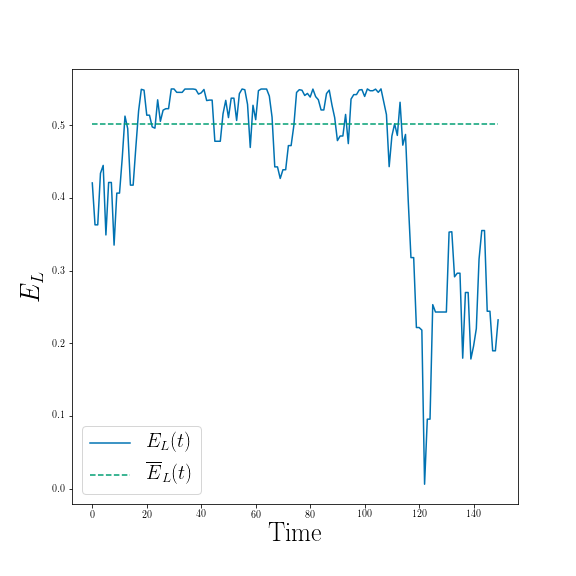
\includegraphics[width=0.8\linewidth]{../results/time-series-example.png}
    \caption{Example time series of local energy values obtained from a
    simulation using Algorithm~\ref{alg:metropolis-simple}. Energies shown
    are a small snippet of energies obtained for a system of one boson in one
    dimension, using $\alpha=0.55$ and a step size of $1$. The mean from the entire set of samples is shown for reference}
    \label{fig:time-series-example}
\end{figure*}

The effect of this is that using \eqref{eq:SE-est-def} directly as the measure for
the statistical error will tend to \textit{underestimate} its true value.

\subsection{Adjusting for Correlated Samples}

We can make the error estimate in \eqref{eq:SE-est-def} less biased by replacing
the sample variance by the sample \textit{covariance}:
\begin{align}
    \begin{split}
        \hat{\sigma}_{\bar{ E_L}} &= \sqrt{\frac{\text{Cov}(E_L)}{n}}\\
        &= \sqrt{\frac{1}{n^2}\sum_{i,j}\qty(E_{L,i} - \bar{E}_L)\qty(E_{L,j}-\bar{E}_L)},
    \end{split}
    \label{eq:SE-est-covar-def}
\end{align}
which we can rewrite in terms of the uncorrelated and correlated contributions
to the error as follows:
\begin{align}
    \begin{split}
    \hat{\sigma}^2_{\bar{E_L}} &=
        \frac{\hat{\sigma}^2_{E_L}}{n}
    + \frac{2}{n^2}\sum_{i<j}\qty(E_{L,i} - \bar{E}_L)\qty(E_{L,j}-\bar{E}_L).
    \end{split}\label{eq:SE-est-covar-expanded}
\end{align}
We observe that if the energies are uncorrelated in time, we would just get back
\eqref{eq:SE-est-def}.

To simplify the notation on the way to the end result, we define following two 
functions:
\begin{gather}
    f_d = \frac{1}{n-d}\sum_{k=1}^{n-d} \qty(E_{L,k} -
    \bar{E}_L)\qty(E_{L,k+d}-\bar{E}_L)\\
    \kappa_d = \frac{f_d}{\hat{\sigma}^2_{E_L}}.
\end{gather}
The function $f_d$ describes the correlation of samples spaced by $d$. We have
$f_0=\sigma_{E_L}^2$, and for an uncorrelated system we have $f_d=0\
\forall\ d>0$.

Now \eqref{eq:SE-est-covar-expanded} can be written as
\begin{align}
    \begin{split}
    \hat{\sigma}^2_{\bar{E_L}} &= \frac{\hat{\sigma}^2_{E_L}}{n} +
    \frac{2\hat{\sigma}^2_{E_L}}{n}\sum_{d=1}^{n-1}\kappa_d\\
    &= \frac{\tau}{n}\ \hat{\sigma}^2_{\bar{E_L}},
    \end{split}
\end{align}
where we have defined the \textit{autocorrelation time} $\tau$, 
\begin{align}
    \tau = 1 + 2\sum_{d=1}^{n-1}\kappa_d,\label{eq:autocorr-time-def}
\end{align}
which can be interpreted as the spacing between samples for which we no longer
observe any correlation. For a completely uncorrelated sample set we have $\tau
=1$, which again results in \eqref{eq:SE-est-def}. Also, any $\tau>1$ will lead
to an \textit{increase} in the estimated error.

This new estimate of the error will be a much more realistic estimate. However,
computing the autocorrelation time $\tau$ has time complexity $\mathcal{O}(n^2)$, which will prove
unfeasible when we plan on producing millions of samples.

\subsection{Methods for Improving the Error Estimate}

We look now at two methods of obtaining improved estimates for the standard
error, besides computing the autocorrelation time $\tau$ directly.

We will look at two such tools here, 
\begin{inparaenum}[1)]
    \item Bootstrap and
    \item Blocking.
\end{inparaenum}

\subsubsection{Bootstrap}
The best way to improve statistical results is usually to simply generate more
data, as statistical estimates tend towards their true value as the number of
samples grow. So ideally, we would simply generate many more sample sets,
$\{E_L\}_b \qfor b=1, 2, \dots, B$, compute the mean for each and produce a
histogram of the results. That would then, for a sufficiently large $B$, serve as
a good estimate for the probability distribution for $\bar E_L$. We could then
compute the standard deviation of said distribution and call that the standard
error of the mean local energy. This would not strictly address the problem of
correlation directly, but averaging results over more data would lessen the
effect. Also, we would expect the individual sample sets to be uncorrelated with
each other, as long as they had differing random seeds.

In practice this is not feasible though, as producing each set of energies will be a
sizable computational task in it self, and not something we can repeat several
times. This is were Bootstrap comes in. The idea of Bootstrap is to simulate
the production of new sample sets by resampling, with replacement, from the
original data set. From the original set $\{E_L\}_1$ we draw $n$ samples with a
uniform probability to get new sets $\{E_L\}_b\qfor b = 2,3,\dots,B$.

As long as the original data set is a representative sample of the space of
energy values (i.e. not biased towards large/small values), and we use a large
enough value for $B$, this will produce a good approximation of the statistical
error. 

This approach has to main limitations. First, it is computationally
expensive to do when the size of the data set is very large, and we need a large
$B$ value.

Second, Bootstrap is still meant to be used on iid. samples, and any estimates
for the error we get from it will still be an underestimate. This comes from the
fact that the original sample set won't be a fully representative sample of the
space, due to the correlations within it. Using Bootstrap will improve the
estimate, but it will still be biased.


\subsection{Blocking}

In some sense Blocking takes the complete opposite approach to that of
Bootstrap. Blocking takes the original samples and combines them to make less
data points.

The idea is to group consecutive samples into \textit{blocks} of a size such
that sample $i$ in block $j$ is uncorrelated with sample $i$ in block $j+1$.
Then, treating each block as a single sample (i.e. by computing the average
energy in each block), we have independent samples of the mean. 

The only issue with this approach is determining how large the blocks need to be
in order for the blocks to become independent. A natural choice would be the
autocorrelation time $\tau$, but that just brings us back to the original
problem of computational infeasibility.

A simple, empirical solution to finding a suitable block size is to make a plot
of the standard deviation of the block means as a function of block
size. Because correlated samples meant we \textit{underestimated} the error (aka.
standard deviation of the sample mean), increasing the block size (i.e. making the
samples less correlated) should increase the observed error. This would keep
going until the block size is so large that the samples have become independent,
at which points it should plateau. Choosing the block size at the plateau point
would then be optimal.

Even better would be an automated way to determine the ideal block size. Such
methods do exists, and will for simplicity be used in this project, although the
manual way would work. The derivation of how this
works, however, will not be discussed any further in this report.


\section{Results for Non-Interacting System}

\subsection{Standard Metropolis Sampling}

\subsubsection{Comparison of Configurations of Parameters}

We now apply the standard Metropolis sampling algorithm described in 
Algorithm\ref{alg:metropolis-simple} to a variety of different settings.
Table~\ref{tab:simple-metro} shows selected results obtained using
$\alpha=\flatfrac{1}{2}$, which corresponds to running with the exact
wavefunction. 

We see that all the results have $\expval{E_L}$
equal (within numerical precision) to the exact result, following
\eqref{eq:exact-ground-state}. In addition, the variance is also equal to
or extremely close to zero, as we expect to observe when we use the correct form
for the exact wavefunction. This is strong evidence that the codes developed are
correct, at least for the non-interacting case.

We see a rather strong dependence on the step size used in the acceptance rates.
It appears we need smaller step sizes when $N$ increases. We would like to tune 
the step size such that we have a significant portion accepted, but still not
run up into the$\sim \SI{100}{\percent}$ region. This is because at this point
we are just stuck in one place, with no real movement. This is not an issue in
the ideal case, because the energy here is actually not dependent on the
positions. But as soon as we move out of this ideal case, this will matter a
great deal. We conclude that a step of $1$ works well in most cases, but must be
lowered a bit for systems with $N \geq 100$.

Perhaps most interesting is to look at the time spent on each configuration. If
we compare the running times for $N=100$ and $N=500$ with analytical expressions
turned off, we see the time increasing by a factor of~$\sim 25$, which is the
square of the factor we increased $N$ by. Looking at the expressions involved in
Algorithm~\ref{alg:metropolis-simple}, we see that this is exactly what we would
expect, namely that the algorithm has time complexity $\mathcal{O}(N^2)$.

Similarly, comparing the run times when analytical expression is turned on, we observe
that time scales as $\mathcal{O}(N)$, resulting in a significantly reduced run
times. It is quite clear that the use of analytic expressions is far superior.
We can, however, expect the difference between the to approaches to be reduced
when we include interaction, as this reduced the analytical approach to the same
complexity as the numerical one.




\subsubsection{Varying the Variational Parameters}

Figure~\ref{fig:var-alpha-plot-noimp} shows a plot of the expected energy, and
corresponding variance, for a $1D$ system of one particle, using $5\cdot 10^4$ Monte
Carlo cycles, as a function of the variational parameter $\alpha$.

We can see a minimum in both graphs, both centered around the ideal value
$\alpha=\flatfrac{1}{2}$. The energy graph is, however, a bit jagged, and the
actual minimum has been found to be a little left of what we would expect. The
curve gets smoother as we increase the number of samples, and extending to
$10^5$ samples yield a {\lq perfect\rq} graph, and this is easily within our
computational reach. The relatively low value of $5\cdot 10^4$ was used to give a visual
difference to the result in the next section, when we include importance
sampling.

\begin{figure*}[ht]
    \centering
    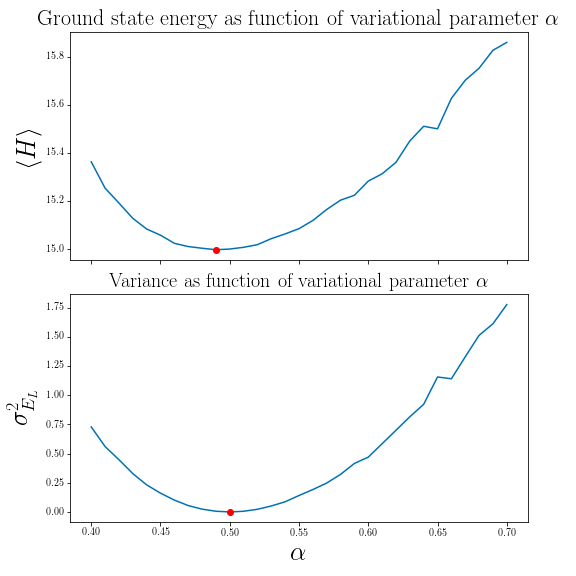
\includegraphics[width=0.9\linewidth]{../results/var-alpha-plot-noimp-50000.png}
    \caption{Plot of average local energy and accompanying population variance,
    as functions of the variational parameter $\alpha$. The minimum of both
    graphs are marked, and is expected to be placed at
    $\alpha=\flatfrac{1}{2}$. Results shown are for $1D$, one particle and
    $5\cdot 10^{4}$ Monte Carlo cycles, using
    Algorithm~\ref{alg:metropolis-simple}.}
    \label{fig:var-alpha-plot-noimp}
\end{figure*}




\subsection{Metropolis-Hastings Sampling}
\subsubsection{Comparison of Configurations of Parameters}

We now apply the improved Metropolis-Hastings sampling algorithm described in 
Algorithm\ref{alg:metropolis-importance} to a variety of different settings.
Table~\ref{tab:importance-metro} shows selected results obtained using
$\alpha=\flatfrac{1}{2}$, which corresponds to running with the exact
wavefunction. 

We see once again that all the results have $\expval{E_L}$
equal (within numerical precision) to the exact result, and very low variance,
indicating that the implementation works as it should.

Looking at the acceptance rates now we see ~$\sim\SI{100}{\percent}$ acceptance
of new moves, indicating that the proposed moves are quite probable and
therefore more likely to be accepted by the sampling algorithm. When $\Delta t$
is to large, however, the result become unstable, as before. At this point the
randomness in \eqref{eq:Langevin-solution} dominates, with steps larger than
what allows for convergence. We may tune this parameter as we wish, so choosing
a value that is small enough for the acceptance rate to be close to one, but
also not so small that we would need an excessive amount of MC cycles in order
to have any exploration in space. We will once again have to tune this parameter
depending on what system we look at, as we need a smaller step for larger
systems.

The run times reported have not changed in any significant way, as would be
expected, as adding importance sampling did not change the complexity of the algorithm.


\subsubsection{Varying the Variational Parameters}
Figure~\ref{fig:var-alpha-plot-imp} shows a plot of the expected energy, and
corresponding variance, for the same system and number of MC cycles as that
shown in Figure~\ref{fig:var-alpha-plot-noimp}. In this version we have enabled
importance sampling.

We can see a very similar result as before, with the notable exception that the
line is less jagged. This implies that the sampling results are more stable.
This is due to the improved exploration of the integration space which
importance sampling gives us. We conclude therefore that the improved algorithm
allows us better, more stable results, compared with the simple sampler. This
allows us to compute less MC samples in order to obtain good enough results,
something which is highly desired for an application where we are constantly
fighting against the large time complexity of this kind of system.

\begin{figure*}[ht]
    \centering
    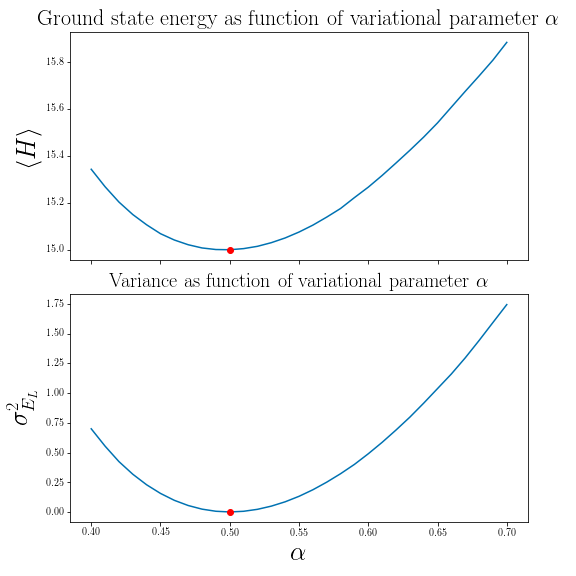
\includegraphics[width=0.9\linewidth]{../results/var-alpha-plot-imp-50000.png}
    \caption{Plot of average local energy and accompanying population variance,
    as functions of the variational parameter $\alpha$. The minimum of both
    graphs are marked, and is expected to be placed at
    $\alpha=\flatfrac{1}{2}$. Results shown are for $1D$, one particle and
    $5\cdot 10^{4}$ Monte Carlo cycles, using
    Algorithm~\ref{alg:metropolis-importance}}
    \label{fig:var-alpha-plot-imp}
\end{figure*}


To get a better view of the effect of $\Delta t$ on the Metropolis-Hastings
sampling algorithm, Figure~\ref{fig:var-alpha-plot-imp-dts} shows the same graph
as before, but for a set of different values for $\Delta t$. From this plot it
becomes very clear that choosing the correct value for this parameter will be
very important when we try to find the optimal variational parameters. We see
that the apparent minima appear on both the left and the right of the ideal
value. 

All values are to some extent usable given enough MC samples, but an unrealistic
number might be needed for $\Delta t$ values far away from the optimum.
Figure~\ref{fig:var-alpha-plot-imp-dts} provides further evidence that $\Delta
t$ must be chosen with care.

\begin{figure*}[ht]
    \centering
    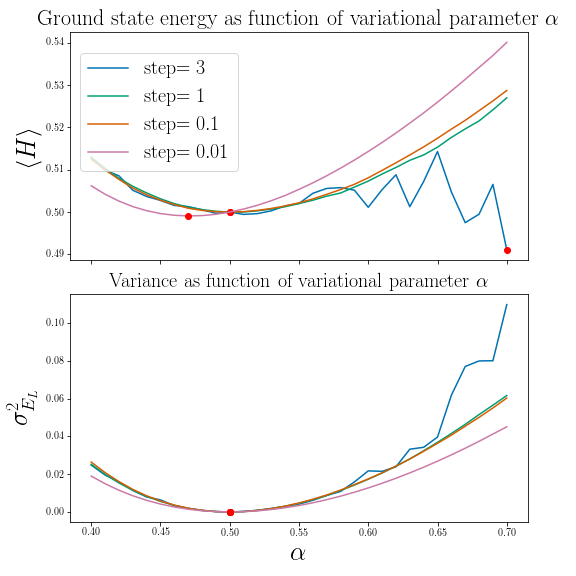
\includegraphics[width=0.9\linewidth]{../results/var-alpha-plot-imp-dts-50000.png}
    \caption{The same plot as shown in Figure~\ref{fig:var-alpha-plot-imp},
    shown for multiple different values for $\Delta t$. We see that both too
    large, and to small values yield less than ideal results.}
    \label{fig:var-alpha-plot-imp-dts}
\end{figure*}

\subsection{Statistical Error}

Figure~\ref{fig:errorbar} shows the results of a simulation on a system of one
boson in 3D, using $n=2^{14}$ Monte Carlo samples. On the graph, error bars are
included to visually express the certainty with which we know the results. The
magnitude of the error bars are given by the standard error, as determined by
the Blocking method. We see that the error estimate goes promptly to zero as we
approach the optimal $\alpha=\flatfrac{1}{2}$ value, and in fact we get exactly
zero as the standard error at this point. This is not that surprising, as using
the optimal value for $\alpha$ here means we are solving the exact system, and
therefore there should not be any doubt about the answer either.

The error estimates might be of higher importance as we traverse into the
interacting case.
\begin{figure*}[ht]
    \centering
    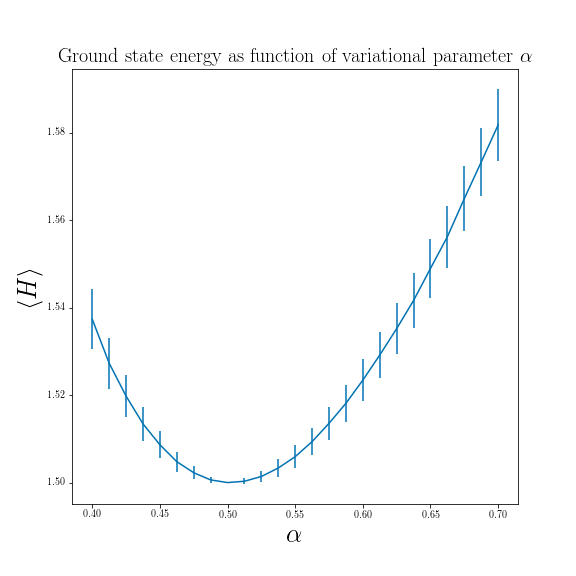
\includegraphics[width=0.8\linewidth]{../results/error-plot-3D-2-pow-14.png}
    \caption{Simulation results using Algorithm~\ref{alg:metropolis-importance},
    running on a system of one boson in 3D, with $\Delta t=0.1$. Error bars have
    been included, whose
    magnitude are the standard error of the mean energy, as obtained by the
    blocking method. In this simulation, $n=2^{14}$ Monte Carlo samples were
    generated.}
    \label{fig:errorbar}
\end{figure*}

\subsection{One-Body Density}

It is also interesting to see how the calculated one-body density comes out for
the ideal non-interacting case. Figure~\ref{fig:density-ideal} shows the plot
for a system of 10 bosons in the 3D symmetric harmonic oscillator trap. Also
drawn is the expected shape from \eqref{eq:one-body-exact}. Both lines have been
normalized so that they integrate to one, as the constants are irrelevant to us
here. To our delight the approximation agrees very well with the expectation.
The discrepancies around $r=0$ are due the volumes of the smallest regions being
very small, and hence their occupation counts become somewhat unstable. We can
still make out the trend though, which again is in great agreement with the
analytical result.

\begin{figure*}[ht]
    \centering
    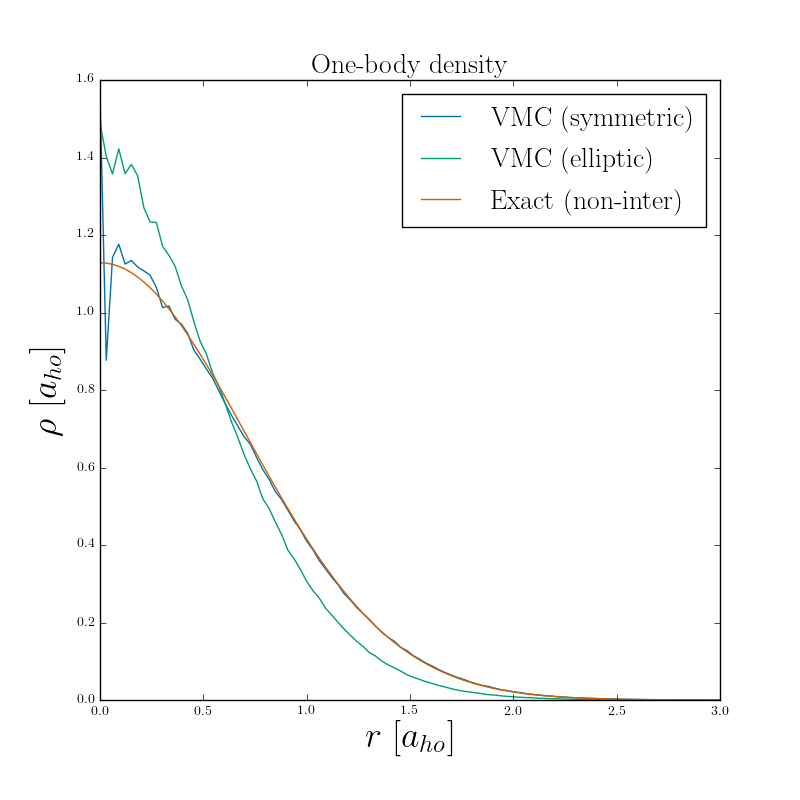
\includegraphics[width=0.8\linewidth]{../results/one-body-3D-N10-noniter.png}
    \caption{One-Body density for a particle in a non-interacting system of 10
    bosons in the 3D symmetric harmonic oscillator trap. The results are with
    $\alpha=\flatfrac{1}{2}$, using Algorithm~\ref{alg:metropolis-simple} with a
    step length of $1$ and $10^6$ samples. For reference is the exact Gaussian
    form expected. Both graphs have been normalized so that they integrate to 1.
    The jagged shape around $r=0$ is an artifact of the approximation used,
    where the volume of the regions become very small, and their counts become
    less stable as a result. The $r$-axis is given in units of $a_{ho}$, and $\rho$ is
    similarly dimensionless.}
    \label{fig:density-ideal}
\end{figure*}


\section{Results for Interacting System}

We now turn our attention to the elliptical trap with the repulsive interaction
activated. We shall in this report fix $\flatfrac{a}{a_{ho}}=0.0043$, and
$\beta=\gamma=2.82843\simeq\sqrt{8}$, as done in \cite{DuBois-phys-rev,
Nilsen-phys-rev}.

\printbibliography


\onecolumn
\begin{center}
\begin{longtable}{|c|c|c|c|c|c|c|c|}
    \caption{Selected results using the standard Metropolis sampling algorithm.
    All runs have been made with $\alpha=\flatfrac{1}{2}$, $\beta=1$, with a
    symmetric trap with strength $\omega_{ho}=1$ and 1000 MC cycles.}
    \label{tab:simple-metro}\\

\hline 
    \multicolumn{1}{|c|}{Analytic} &
    \multicolumn{1}{c|}{Dimensions} &
    \multicolumn{1}{c|}{Particles} &
    \multicolumn{1}{c|}{Step length} &
    \multicolumn{1}{c|}{$\expval{H}$} &
    \multicolumn{1}{c|}{$\text{Var}(E_L)$} &
    \multicolumn{1}{c|}{Acceptance Rate} &
    \multicolumn{1}{c|}{Time (s)}  \\ \hline
\endfirsthead

\multicolumn{8}{c}%
{{\bfseries \tablename\ \thetable{} -- continued from previous page}} \\
\hline 
    \multicolumn{1}{|c|}{Analytic} &
    \multicolumn{1}{c|}{Dimensions} &
    \multicolumn{1}{c|}{Particles} &
    \multicolumn{1}{c|}{Step length} &
    \multicolumn{1}{c|}{$\expval{H}$} &
    \multicolumn{1}{c|}{$\text{Var}(E_L)$} &
    \multicolumn{1}{c|}{Acceptance Rate} &
    \multicolumn{1}{c|}{Time (s)} \\ \hline
\endhead

\hline \multicolumn{8}{|r|}{{Continued on next page}} \\ \hline
\endfoot

\hline
\endlastfoot

\csvreader[head to column names]{../results/vmc_configurations.csv}{}
    {\csvcoliii & \csvcoli & \csvcolii & \csvcoliv & \csvcolv & \csvcolvi &
    \csvcolvii & \csvcolviii\\}

\end{longtable}
\end{center}
\begin{center}
\begin{longtable}{|c|c|c|c|c|c|c|c|}
    \caption{Selected results using improved Metropolis-Hastings sampling algorithm.
    All runs have been made with $\alpha=\flatfrac{1}{2}$, $\beta=1$, with a
    symmetric trap with strength $\omega_{ho}=1$ and 1000 MC cycles.}
    \label{tab:importance-metro} \\

\hline 
    \multicolumn{1}{|c|}{Analytic} &
    \multicolumn{1}{c|}{Dimensions} &
    \multicolumn{1}{c|}{Particles} &
    \multicolumn{1}{c|}{$\Delta t$} &
    \multicolumn{1}{c|}{$\expval{H}$} &
    \multicolumn{1}{c|}{$\text{Var}(E_L)$} &
    \multicolumn{1}{c|}{Acceptance Rate} &
    \multicolumn{1}{c|}{Time (s)}  \\ \hline
\endfirsthead

\multicolumn{8}{c}%
{{\bfseries \tablename\ \thetable{} -- continued from previous page}} \\
\hline 
    \multicolumn{1}{|c|}{Analytic} &
    \multicolumn{1}{c|}{Dimensions} &
    \multicolumn{1}{c|}{Particles} &
    \multicolumn{1}{c|}{$\Delta t$} &
    \multicolumn{1}{c|}{$\expval{H}$} &
    \multicolumn{1}{c|}{$\text{Var}(E_L)$} &
    \multicolumn{1}{c|}{Acceptance Rate} &
    \multicolumn{1}{c|}{Time (s)} \\ \hline
\endhead

\hline \multicolumn{8}{|r|}{{Continued on next page}} \\ \hline
\endfoot

\hline
\endlastfoot

\csvreader[head to column names]{../results/vmc_imp_configurations.csv}{}
    {\csvcoliii & \csvcoli & \csvcolii & \csvcoliv & \csvcolv & \csvcolvi &
    \csvcolvii & \csvcolviii\\}

\end{longtable}
\end{center}
\twocolumn



\end{document}
